\chapter{Text detection}
\label{chap:text-detection}


\section{Introduzione}
Negli ultimi anni, con l'avvento delle tecnologie di intelligenza artificiale e machine learning, gli algoritmi di rilevamento e riconoscimento del testo (\textit{text detection and recognition}) hanno subito un'evoluzione radicale, sia dal punto di vista dell'accuratezza dei risultati che dal punto di vista del tempo di esecuzione. Per quanto riguarda la \textit{text recognition} basta osservare il salto di qualit\`a subito da motori OCR open-source, quali \textit{Tesseract}, a seguito dell'implementazione di reti neurali ricorrenti (\textit{RNN}) di tipo \textit{LSTM} (\textit{Long Short Term Memory}), particolarmente adatte per questo tipo di applicazioni.\par
In questo capitolo ci concentriamo sull'introduzione di alcuni algoritmi di \textit{text detection}, che vengono utilizzati per riconoscere regioni di testo presenti in un'immagine e presentiamo un integrazione efficiente di questi metodi all'interno della libreria QI-OCR. 


\section{MSER}
Il metodo presentato in \cite{bib:mser} \`e un algoritmo di \textit{blob\footnote{Un blob in un'immagine \`e un gruppo connesso di pixel che condividono una determinata propriet\`a.} detection}, per la rilevazione di alcuni regioni distinguibili (\textit{DRs - Distinguished Regions}) in un'immagine, ovvero regioni che posseggono propriet\`a di stabilit\`a e invarianza, con un conseguente alto grado di ripetibilit\`a nella rilevazione.\par
Introduciamo delle regioni che vengono denominate \textit{ER (Extremal Regions)}, nel senso che tutti i pixel interni hanno intensit\`a esclusivamente maggiore o minore dei pixel nel contorno esterno della regione. Le \textit{ER} godono di due importanti propriet\`a: sono invarianti per trasformazioni geometriche affini e per trasformazioni monot\`one di intensit\`a dell'immagine. Le regioni di interesse sono un sottoinsieme delle \textit{ER} e vengono denominate \textit{MSER} (\textit{Maximally Stable Extremal Regions}), poich\`e risultano \textit{stabili} sotto una serie di operazioni di \textit{thresholding} e permettono una rilevazione multi-scala delle regioni, nel senso che vengono individuate sia strutture molto piccole che molto grandi.\par
Il grande vantaggio di questo \textit{blob detector} \`e la sua efficienza, in quanto l'enumerazione di tutte le \textit{ER} ha una complessit\`a temporale quasi lineare\footnote{In \cite{bib:mser-linear} \textit{Nist\'er} e \textit{Stew\'enius} propongono un metodo per l'enumerazione delle \textit{MSER} in tempo $\mathcal{O}(n)$, lineare nel numero di pixel dell'immagine.} di $\mathcal{O}(n\log{}\log{}n)$, data principalmente dall'algoritmo di enumerazione delle componenti connesse\footnote{Esiste una versione pi\`u efficiente, ma pi\`u articolata, dell'algoritmo per il \textit{labeling} delle componenti connesse (\textit{Rosenfeld-Pfaltz} \cite{bib:connected-components-fast}) con complessit\`a $\mathcal{O}(n\alpha(n))$, con $\alpha$ inversa della funzione di \textit{Ackermann}.}, con $n$ numero di pixel dell'immagine.\par
Nella pratica, l'algoritmo presentato pu\`o essere adattato per vari scopi e in particolare per il riconoscimento di testo in ambienti naturali, come descritto in \cite{bib:mser-canny}.\par
In figura \ref{fig:mser} un esempio di \textit{text detection} con l'utilizzo dell'algoritmo \textit{MSER} implementato nella libreria \textit{OpenCV}:
\begin{figure}[h]
	\centering
	\resizebox{\textwidth}{!}{
		\centering
		\subfloat[Input] {%
			\scalebox{0.5}[0.5] {
				\frame{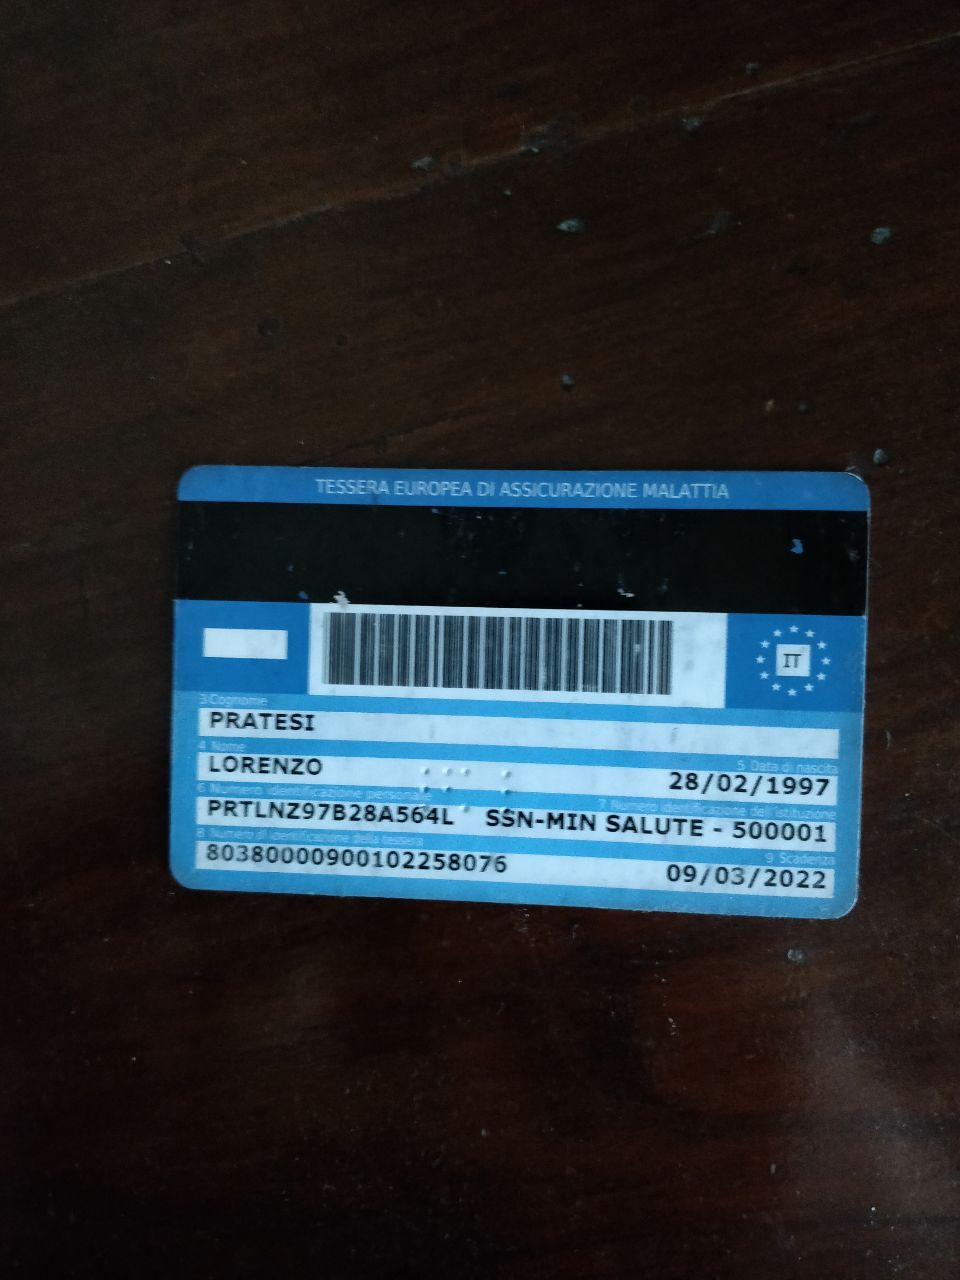
\includegraphics[width=.5\linewidth]{img/mser-east-input.png}}
			}
		}
		\subfloat[Output] {%
			\scalebox{0.5}[0.5] {
				\frame{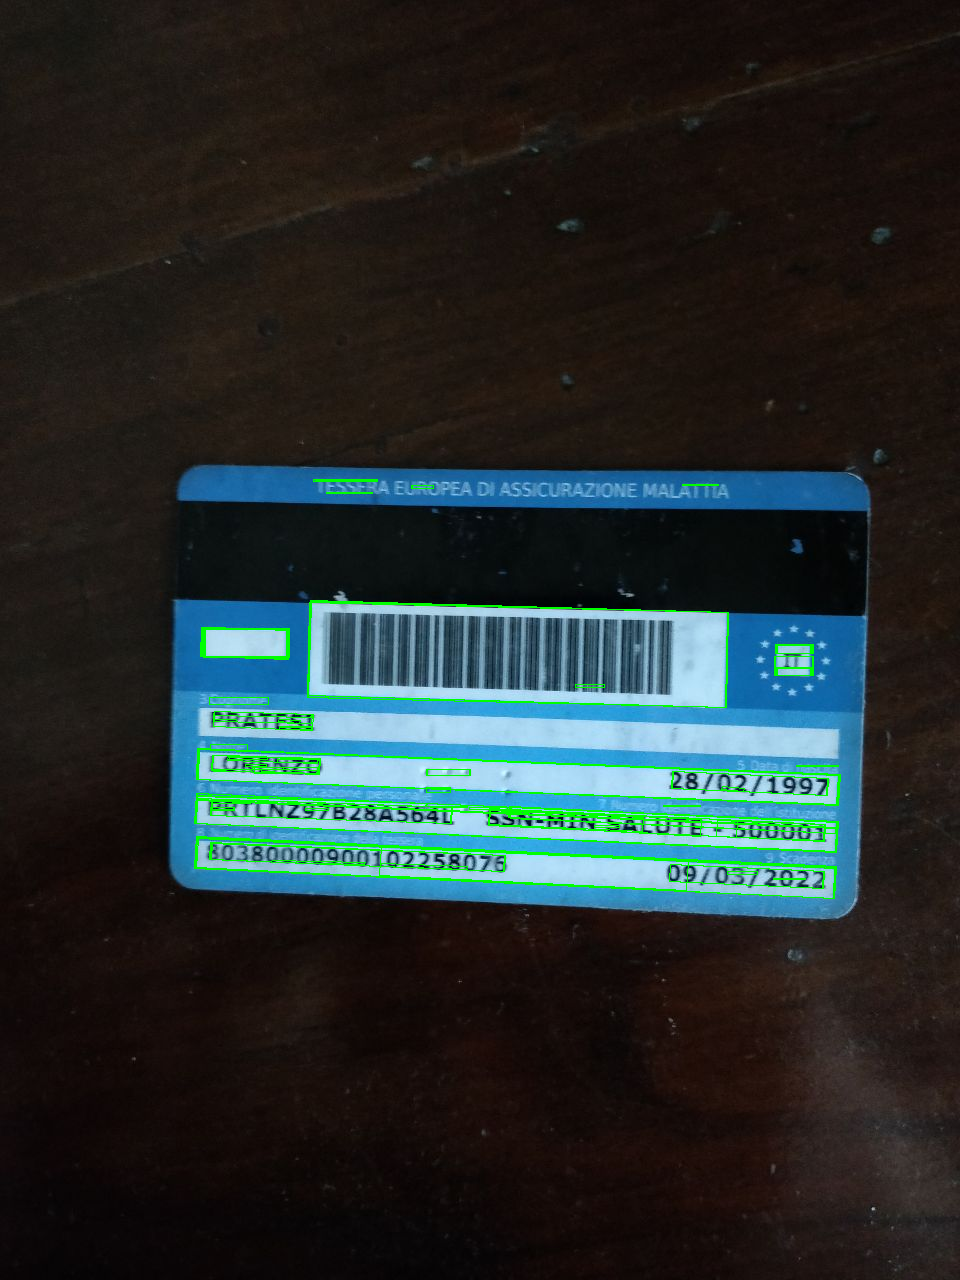
\includegraphics[width=.5\linewidth]{img/mser-regions.png}}
			}
		}
		\subfloat[][Output filtrato] {%
			\scalebox{0.5}[0.5] {
				\frame{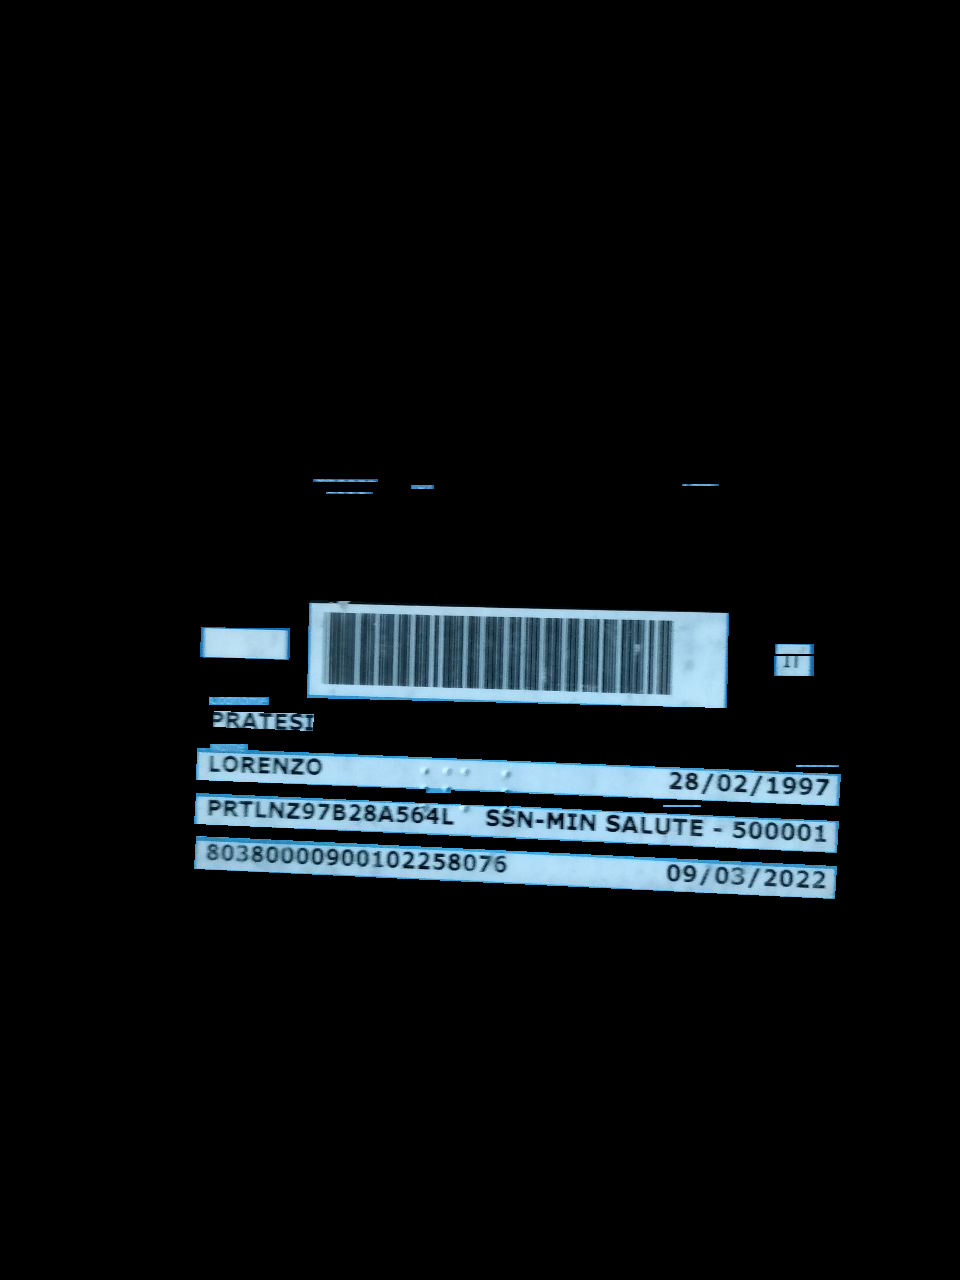
\includegraphics[width=.5\linewidth]{img/mser-regions-filtered.png}}
			}
		}
	}
	\caption{\textit{Text detection} con \textit{MSER}} \label{fig:mser}
\end{figure}


\section{EAST}
L'approccio ideale per i problemi di \textit{text detection} sarebbe quello di utilizzare un algoritmo che prende in input un'immagine e restituisce una lista di rettangoli, in cui ciascun rettangolo identifica una regione di testo dell'immagine. In base al tipo di \textit{text detection} che si intende effettuare, non orientata o orientata, ciascun rettangolo \`e identificato, rispettivamente, da una coppia $(x, y)$, $lunghezza$ e $altezza$, oppure da 4 coppie $(x, y)$ per ciascun vertice del rettangolo. Osservando l'output prodotto da \textit{MSER} in figura \ref{fig:mser}, \`e possibile constatare che le regioni restituite non sono solamente quelle contenenti testo. Infatti, nell'esempio riportato, viene evidenziata anche la regione contenente il \textit{codice a barre} del documento.\par 
\textit{EAST} (\textit{Efficient and Accurate Scene Text detector}) \cite{bib:east} cerca di superare i limiti di \textit{blob detector} come \textit{MSER}, tramite l'implementazione di una rete neurale convoluzionale (\textit{FCN - Fully Convolutional Network}). Le specifiche di questa soluzione non rientrano negli obiettivi di questa tesi, ma nelle figure \ref{fig:mser} e \ref{fig:east} presentiamo un esempio di immagine processata sia da \textit{MSER} che dalla rete \textit{EAST}, per poter confrontare i risultati ottenuti.
\begin{figure}[h]
	\centering
	\resizebox{\textwidth}{!}{
		\centering
		\subfloat[Input] {%
			\scalebox{0.5}[0.5] {
				\frame{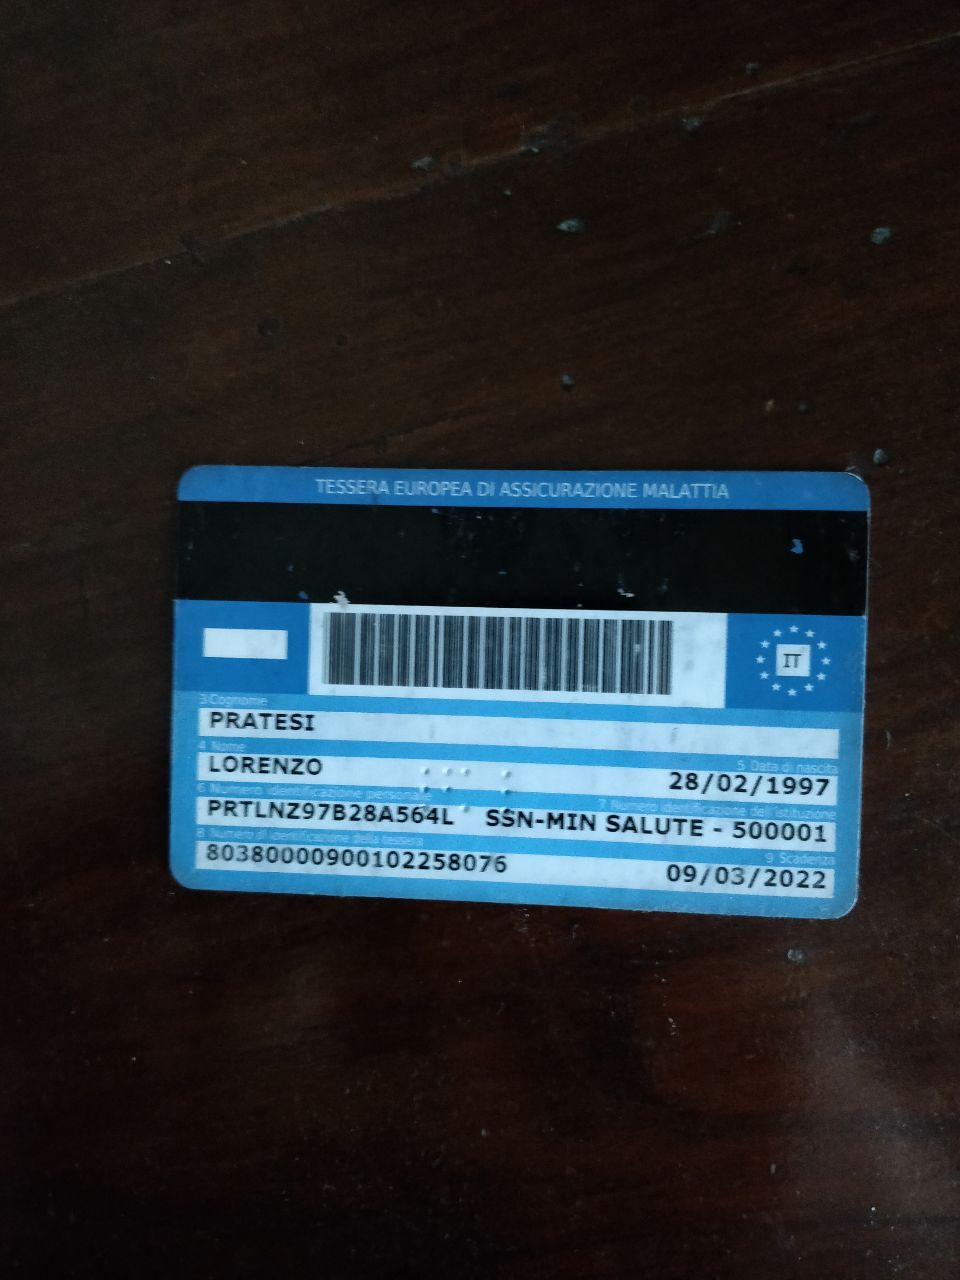
\includegraphics[width=.8\linewidth]{img/mser-east-input.png}}
			}
		}
		\subfloat[Output] {%
			\scalebox{0.5}[0.5] {
				\frame{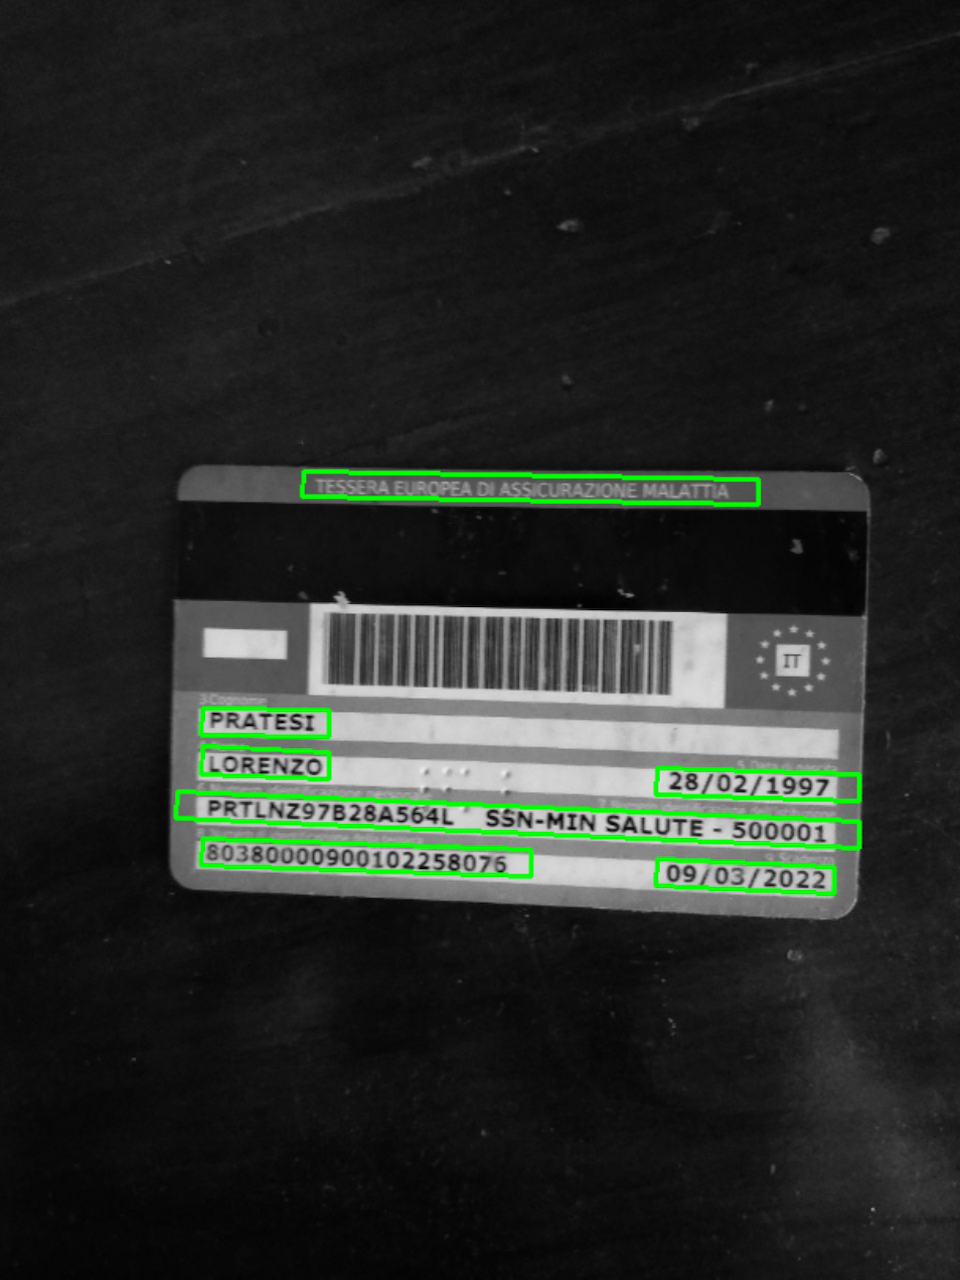
\includegraphics[width=.79\linewidth]{img/east-output.png}}
			}
		}
	}
	\caption{\textit{Text detection} con \textit{EAST}} \label{fig:east}
\end{figure}


\section{Ritaglio dinamico dei campi di un documento}
In questa sezione presentiamo un approccio dinamico per il ritaglio dei campi di un documento d'identit\`a. Prima dell'introduzione di questo metodo, la libreria QI-OCR effettuava un ritaglio statico per ogni campo del documento in analisi, in base a coordinate predeterminate dal \textit{template} del documento e ipotizzando un ritaglio e una centratura quasi perfetta a seguito degli algoritmi di localizzazione descritti nel capitolo \ref{chap:image-matching}.\par
In tabella \ref{tab:car-r-coords} un esempio di coordinate definite per il retro della vecchia carta d'identit\`a italiana, in base a una dimensione di $700 \times 1000$ pixel, con campi e template visibili in figura \ref{fig:car-r-template}.\par
\begin{figure}[h]
	\centering
	\resizebox{.4\textwidth}{!}{
		\centering
		\begin{tikzpicture}
			\draw[->,ultra thick] (0,5)--(3.6,5) node[right]{$x$};
			\draw[->,ultra thick] (0,5)--(0,0) node[below]{$y$};
			
			\hspace*{0.2cm}
			\scalebox{0.5}[0.5] {
				\frame{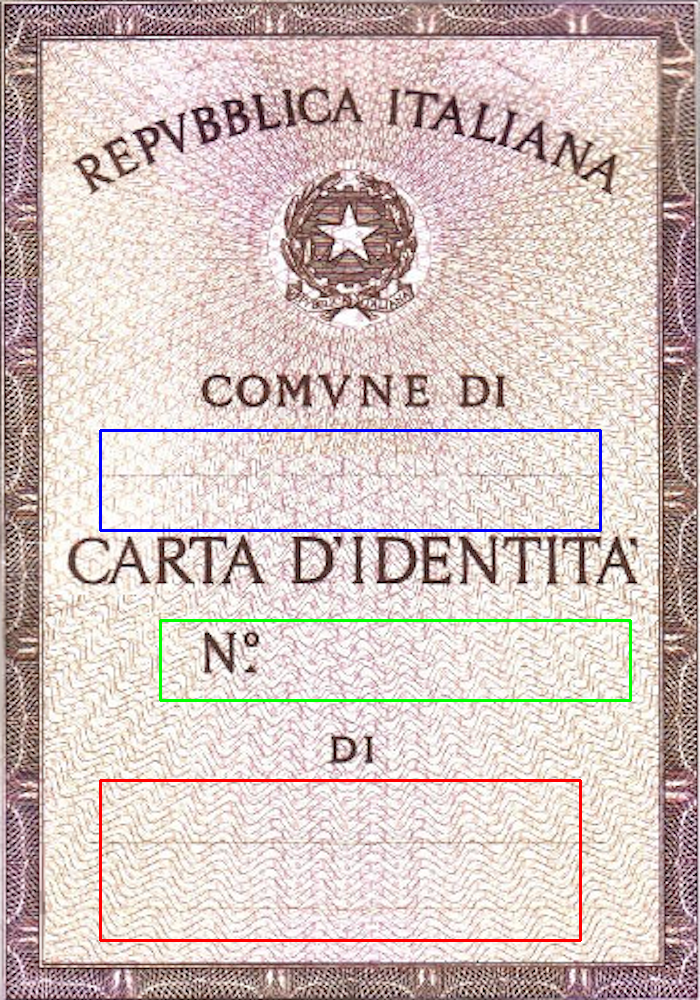
\includegraphics[width=.5\linewidth]{img/car-r-fields.png}}
			}
		\end{tikzpicture}
	}
	\caption{Campi vecchia carta d'identit\`a italiana (retro)} \label{fig:car-r-template}
\end{figure}
\begin{table}[H]
	\centering
	\resizebox{.8\textwidth}{!}{%
	\begin{tabular}{|c|c|c|c|c|}
	\hline
	\textbf{Campo} & \textbf{$x$} & \textbf{$y$} & \textbf{$larghezza$} & \textbf{$altezza$} \\ \hline
	{\color{blue}Comune} & $100px$ & $430px$ & $500px$ & $100px$ \\ \hline
	{\color{green}Numero documento} & $160px$ & $620px$ & $470px$ & $80px$ \\ \hline
	{\color{red}Nome completo} & $100px$ & $780px$ & $480px$ & $160px$ \\ \hline
	\end{tabular}%
	}
	\caption{Coordinate campi vecchia carta d'identit\`a italiana (retro)}
	\label{tab:car-r-coords}
\end{table}
Purtroppo, con il ritaglio statico utilizzato il rischio di perdita d'informazione aumenta quando la localizzazione del documento ritorna un risultato approssimativo, oppure quando si stanno estraendo campi da documenti che non rispettano esattamente i template prefissati, come la vecchia carta d'identit\`a italiana. Per avere un'idea pi\`u concreta della problematica menzionata, in figura \ref{fig:car-f-example} mostriamo un esempio di carta d'identit\`a cartacea che non rispetta gli standard e in figura \ref{fig:car-f-static} i relativi campi ritagliati in modo statico.\par
\begin{figure}[H]
	\centering
	\resizebox{.6\textwidth}{!}{
		\frame{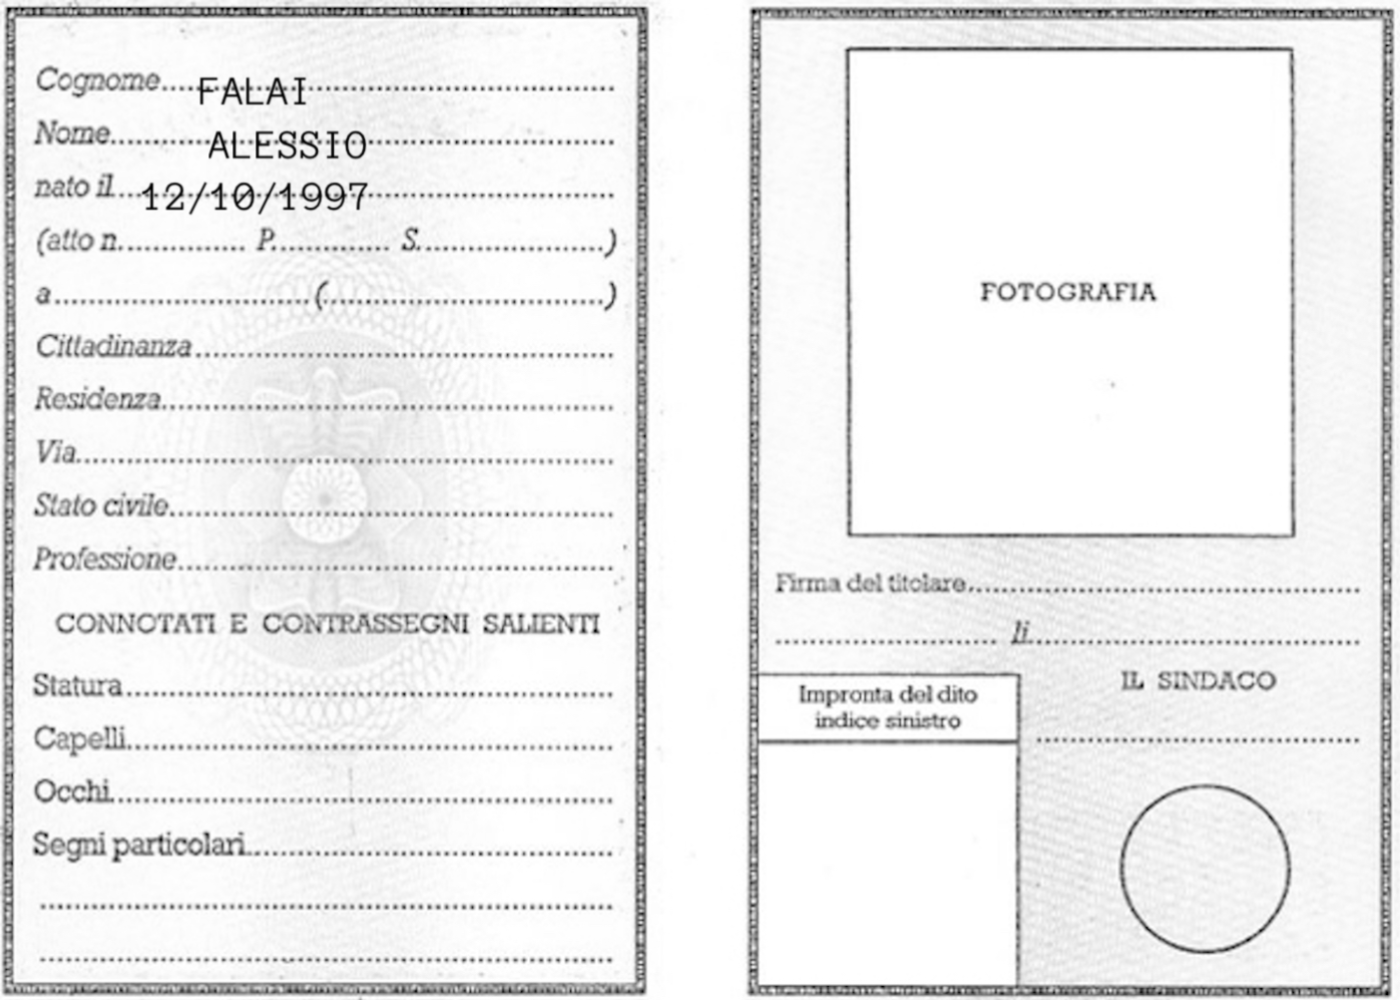
\includegraphics[]{img/car-f.png}}
	}
	\caption{Vecchia carta d'identit\`a italiana (fronte) non standard} \label{fig:car-f-example}
\end{figure}
\begin{figure}[h]
	\centering
	\resizebox{\textwidth}{!}{
		\centering
		\subfloat[Nome] {%
			\scalebox{0.5}[0.5] {
				\frame{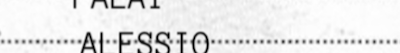
\includegraphics[width=.5\linewidth]{img/car-f-name-static.png}}
			}
		}
		\subfloat[Cognome] {%
			\scalebox{0.5}[0.5] {
				\frame{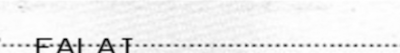
\includegraphics[width=.5\linewidth]{img/car-f-surname-static.png}}
			}
		}
		\subfloat[Data di nascita] {%
			\scalebox{0.5}[0.5] {
				\frame{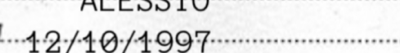
\includegraphics[width=.5\linewidth]{img/car-f-birthdate-static.png}}
			}
		}
	}
	\caption{Campi vecchia carta d'identit\`a italiana (fronte) non standard, ritagliati in modo statico} \label{fig:car-f-static}
\end{figure}
L'approccio proposto consente di risolvere le problematiche del ritaglio statico, quando lo scostamento delle coordinate reali da quelle predefinite non \`e troppo elevato. L'algoritmo in questione prevede l'individuazione delle regioni di testo in modo dinamico, tramite uno degli algoritmi di \textit{text detection} descritti. Dopodich\`e, per ciascun campo, le informazioni sui \textit{bounding boxes dinamici} vengono utilizzate per calcolare il valore di ordinata effettivo e la lunghezza corretta del campo in esame. Per svolgere questo compito, l'algoritmo computa l'intersezione del rettangolo statico con tutti i rettangoli dinamici e calcola l'area di intersezione massima. Le coordinate del \textit{bounding box dinamico} che ha dato l'intersezione di area massima vengono utilizzate per determinare i nuovi valori di $y$ e $lunghezza$ del campo analizzato. Lo pseudocodice della procedura descritta \`e definito nell'algoritmo \ref{alg:dynamic-cut}, mentre l'immagine \ref{fig:car-f-dynamic} mostra i risultati ottenuti nell'esempio riportato in figura \ref{fig:car-f-example}, grazie all'utilizzo della rete \textit{EAST} (vedi figura \ref{fig:car-f-example-east}).
\begin{figure}[H]
	\centering
	\resizebox{.6\textwidth}{!}{
		\frame{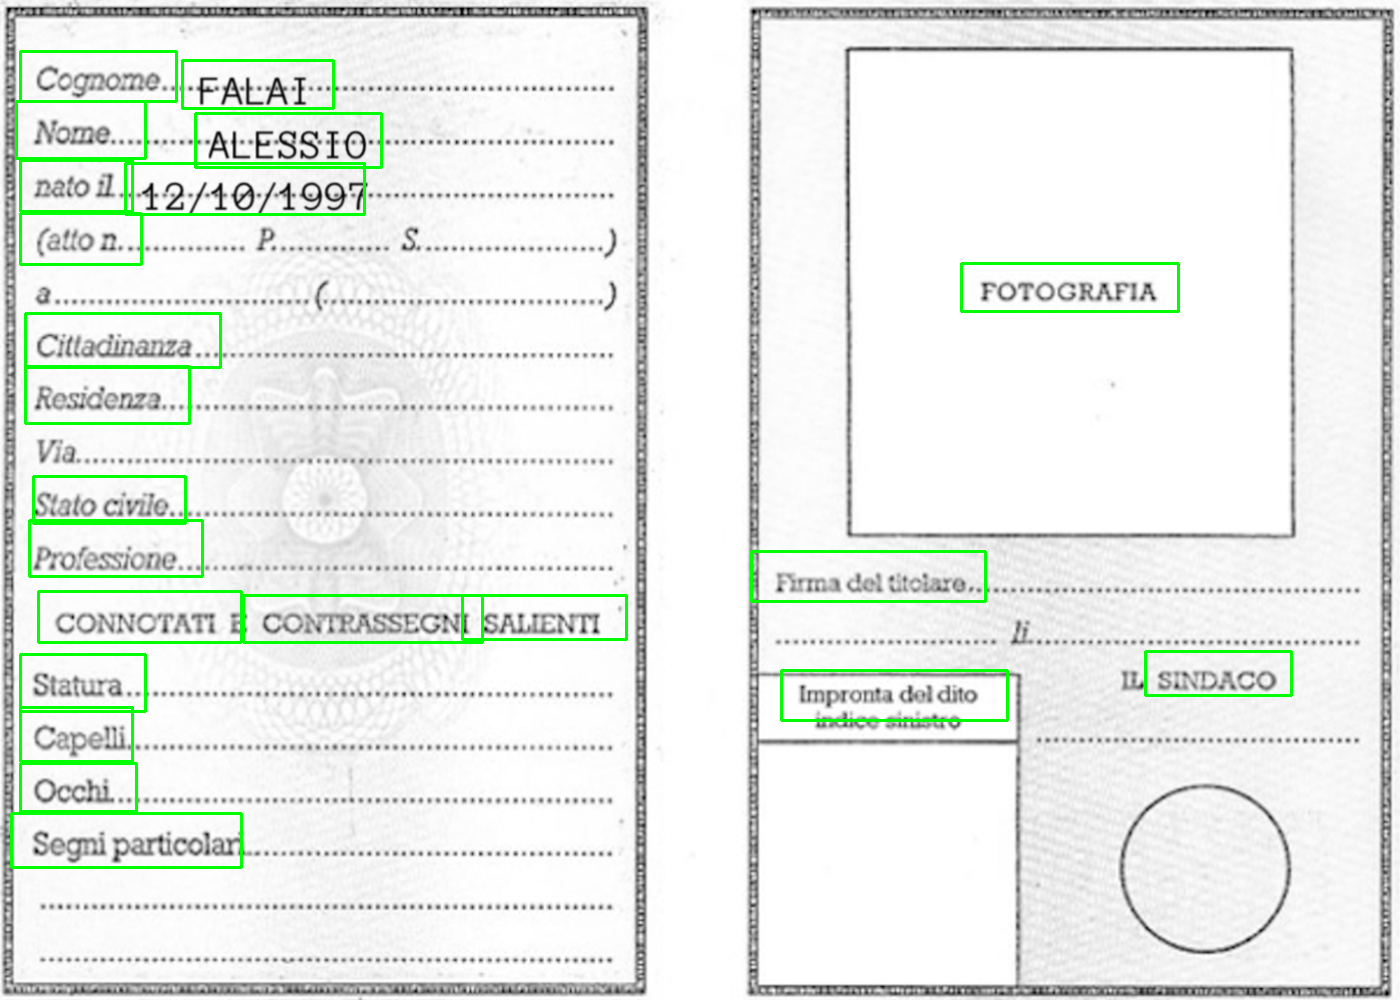
\includegraphics[]{img/car-f-east.png}}
	}
	\caption{Output di \textit{EAST} su una vecchia carta d'identit\`a italiana (fronte) non standard} \label{fig:car-f-example-east}
\end{figure}
\begin{figure}[H]
	\centering
	\resizebox{\textwidth}{!}{
		\centering
		\subfloat[Nome] {%
			\scalebox{0.5}[0.5] {
				\frame{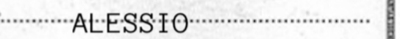
\includegraphics[width=.5\linewidth]{img/car-f-name-dynamic.png}}
			}
		}
		\subfloat[Cognome] {%
			\scalebox{0.5}[0.5] {
				\frame{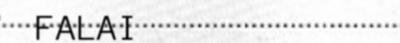
\includegraphics[width=.5\linewidth]{img/car-f-surname-dynamic.png}}
			}
		}
		\subfloat[Data di nascita] {%
			\scalebox{0.5}[0.5] {
				\frame{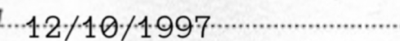
\includegraphics[width=.5\linewidth]{img/car-f-birthdate-dynamic.png}}
			}
		}
	}
	\caption{Campi vecchia carta d'identit\`a italiana (fronte) non standard, ritagliati in modo dinamico} \label{fig:car-f-dynamic}
\end{figure}

\begin{algorithm}[H]
	\caption{Ritaglio dinamico}
	\label{alg:dynamic-cut}
	
	\begin{algorithmic}[1]
		\Function{dynamic-cut}{}
			\State $\vars{image} \gets \text{input image}$
			\State $\vars{field} \gets \text{rectangle} (\vars{x}, \vars{y}, \vars{width}, \vars{height})$
			\State $\vars{dynamic-fields} \gets \text{list of rectangles} (\vars{x}, \vars{y}, \vars{width}, \vars{height})$
			\\
			\State $\vars{max-bbox} \gets \textproc{max-intersection-area-bbox(\vars{field}, \vars{dynamic-fields})}$
			\State $\vars{field.y} \gets \vars{max-bbox.y}$
			\State $\vars{field.width} \gets \textproc{max(\vars{field.width, max-bbox.width})}$

			\Return $\vars{image[field.y:field.y + field.height]}$\newline\hspace*{2.91cm}
					$\vars{[field.x:field.x + field.width]}$
		\EndFunction
		\Statex
		\Function{max-intersection-area-bbox}{}
			\State $\vars{field} \gets \text{rectangle} (\vars{x}, \vars{y}, \vars{width}, \vars{height})$
			\State $\vars{dynamic-fields} \gets \text{list of rectangles} (\vars{x}, \vars{y}, \vars{width}, \vars{height})$
			\\
			\State $\vars{max-area} \gets 0\text{, } \vars{max-bbox} \gets field$
			\For {$\vars{dynamic-field} \text{ in \vars{dynamic-fields}}$}
				\State $\vars{area} \gets \textproc{intersection-area(\vars{field}, \vars{dynamic-field})}$
				\If {$\vars{area} > \vars{max-area}$}
					\State $\vars{max-area} \gets \vars{area}$
					\State $\vars{max-bbox} \gets \vars{dynamic-field}$
				\EndIf
			\EndFor

			\Return $\vars{max-bbox}$
		\EndFunction
		\Statex
		\Function{intersection-area}{}
			\State $\vars{rect-one} \gets \text{rectangle} (\vars{x}, \vars{y}, \vars{width}, \vars{height})$
			\State $\vars{rect-two} \gets \text{rectangle} (\vars{x}, \vars{y}, \vars{width}, \vars{height})$
			\\
			\State $\vars{dx} \gets 0\text{, } \vars{dy} \gets 0$
			
			\State $\vars{dx} = \textproc{min}(\vars{rect-one.x} + \vars{rect-one.width},$\newline\hspace*{0.6cm}$\vars{rect-two.x} + \vars{rect-two.width}) - \textproc{max}(\vars{rect-one.x}, \vars{rect-two.x})$
			\State $\vars{dy} = \textproc{min}(\vars{rect-one.y} + \vars{rect-one.height},$\newline\hspace*{0.6cm}$\vars{rect-two.y} + \vars{rect-two.height}) - \textproc{max}(\vars{rect-one.y}, \vars{rect-two.y})$

			\If {$\vars{dx} > 0 \wedge \vars{dy} > 0$}
				\Return $\vars{dx} \cdot \vars{dy}$
			\EndIf

			\Return $0$
		\EndFunction
	\end{algorithmic}
\end{algorithm}
